\documentclass{standalone}
\usepackage{tikz}
\begin{document}
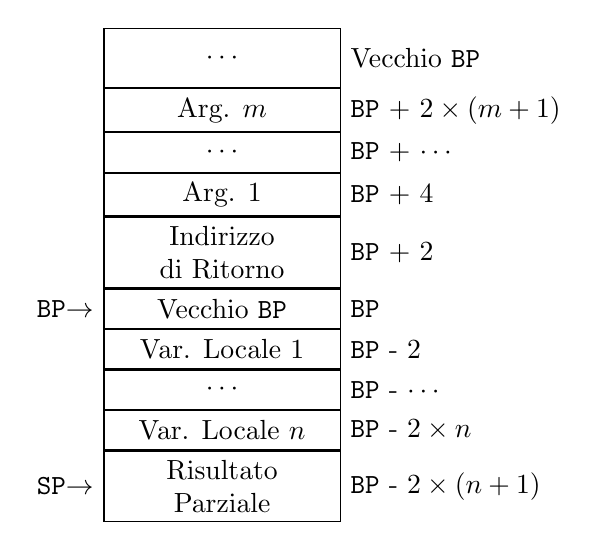
\begin{tikzpicture}
    \draw

    (0,0)node[rectangle,draw,anchor=north,minimum height=0.75cm, minimum width=3cm](a){$\cdots$}
    (a.east)node[right]{Vecchio \verb|BP|}
    (a.south)node[rectangle,draw,anchor=north,minimum height=0.5cm, minimum width=3cm](a){Arg. $m$}
    (a.east)node[right]{\verb|BP| + $2\times (m+1)$}
    (a.south)node[rectangle,draw,anchor=north,minimum height=0.5cm, minimum width=3cm](a){$\cdots$}
    (a.east)node[right]{\verb|BP| + $\cdots$}
    (a.south)node[rectangle,draw,anchor=north,minimum height=0.5cm, minimum width=3cm](a){Arg. 1}
    (a.east)node[right]{\verb|BP| + 4}
    (a.south)node[rectangle,draw,anchor=north,minimum height=0.5cm, minimum width=3cm,align=center](a){Indirizzo\\di Ritorno}
    (a.east)node[right]{\verb|BP| + 2}
    (a.south)node[rectangle,draw,anchor=north,minimum height=0.5cm, minimum width=3cm](a){Vecchio \verb|BP|}
    (a.east)node[right]{\verb|BP|}
    (a.west)node[left]{\verb|BP|$\to$}
    (a.south)node[rectangle,draw,anchor=north,minimum height=0.5cm, minimum width=3cm](a){Var. Locale 1}
    (a.east)node[right]{\verb|BP| - 2}
    (a.south)node[rectangle,draw,anchor=north,minimum height=0.5cm, minimum width=3cm](a){$\cdots$}
    (a.east)node[right]{\verb|BP| - $\cdots$}
    (a.south)node[rectangle,draw,anchor=north,minimum height=0.5cm, minimum width=3cm](a){Var. Locale $n$}
    (a.east)node[right]{\verb|BP| - $2\times n$}
    (a.south)node[rectangle,draw,anchor=north,minimum height=0.5cm, minimum width=3cm,align=center](a){Risultato\\Parziale}
    (a.east)node[right]{\verb|BP| - $2\times (n+1)$}
    (a.west)node[left]{\verb|SP|$\to$}
    
    ;
\end{tikzpicture}
\end{document}